\documentclass[
    paper=A4,
    div=calc,
    numbers=noendperiod
    % twocolumn
]{scrartcl}

% Infos:
% 3 din a4 seiten

\usepackage[utf8]{inputenc}
\usepackage[T1]{fontenc}
\usepackage[ngerman]{babel}
\usepackage{microtype}
\usepackage{libertine}
\usepackage[libertine]{newtxmath}

\usepackage[headsepline]{scrlayer-scrpage}
\usepackage{siunitx}
\usepackage{pdfpages}

\usepackage[
    bookmarksnumbered   =   true,
    breaklinks          =   true,
    colorlinks          =   true,
    pdftitle            =   {Mentoring Jan Hoegen},
    pdfsubject          =   {Mentoring HKA WS 22/23},    
    pdfauthor           =   {Jan Hoegen},
]{hyperref}

\titlehead{Hochschule Karlsruhe\\Univerity of Applied Sciences}
\subject{Studiengang Elektro- und Informationstechnik}
\title{Mentoringbericht Wintersemster 2022/23}
% \subtitle{Wintersemster }
% \author{Jan Hoegen\thanks{Matrikelnummer: 82358. E-Mail: \href{mailto:jan.hoegen@web.de}{jan.hoegen@web.de}}}
\author{Jan Hoegen\\\href{mailto:jan.hoegen@web.de}{jan.hoegen@web.de}}
\date{Erstellt am \today}
% \publishers{xx}

\ihead{Jan Hoegen}
\chead{Mentoringbericht WS 22/23}
\ohead{\today}

\begin{document}

\maketitle

% \tableofcontents

\section{Rahmenbedingungen}
    Das Mentoringprogramm richtet sich an Erstsemesterstudentinnen und -Studenten an der Hochschule Karlsruhe im Studiengang Elektro- und Informationstechnik für das Wintersemster 2022/23. Organisiert wird es vom Zentrum für Lehrinnovation der HKA. Ziel ist es, den Studierenden den Einstieg ins Studium durch erfahrene Kommilitonen zu erleichtern.

    Ich bin 23 Jahre alt, studiere Elektro- und Informationstechnik im zweiten Bachelorsemester, und nehme zum ersten Mal als Mentor an diesem Programm teil. Gemeinsam mit Raphael Hansjosten (6. Bachelorsemester) bilden wir ein Team und betreuen insgesamt elf Mentees. 

    \subsection*{Vorkenntnisse}
        Raphael Hansjosten nimmt zum zweiten Mal als Mentor teil und studiert bereits seit 3 Jahren an der Hochschule, daher kann ich auf seinen großen Erfahrungsschatz und sein hochschulspezifisches Wissen zurückgreifen. 

        Obwohl ich über weniger Erfahrung über das Studium an der HKA verfüge, fühle ich mich dennoch gut vorbereitet, die Mentees in ihrem ersten Semester zu unterstützen. Dank meiner Vorkenntnisse als lizenzierter C-Trainer im Bereich Leistungssport Erwachsene Volleyball bin ich mit den Themen Mehrjahreszielsetzung, Planung und Umsetzung, sowie Wissensvermittlung gegenüber Jugendliche geübt.  
        Aufgrund meiner Werkstudententätigkeit im Rettungsdienst und Krankentransport Karlsruhe bin ich über psychische Probleme und ihre Anlaufstellen zur Selbsthilfe sensibilisiert.  
        
        % Ich bin lizenzierter C-Trainer im Bereich Leistungssport Erwachsene Volleyball, war drei Jahre Übungsleiter und Coach einer U20w im Volleyball und nehme aktuell im Wohnheim ein Amt ein. Außerdem arbeite ich als Werkstudent im Rettungsdienst und Krankentransport in Karlsruhe. Darüber hinaus liegt das erste Semester kurz hinter mir und ich konnte frische Erfahrungen sammeln.
 
\section{Zielsetzung}
    Folgende Aufgaben wurden an die Mentoren formuliert:

    \begin{itemize}
        \item Beratung der Mentees über das erste Semester hinweg geben
        \item Anlaufstelle für Fragen rund um das Studium sein
        \item Wissen und Erfahrung teilen
        \item Fachliche und organisatorische Tipps geben
        \item Mentees motivieren, Entscheidungen eigenständig und reflektiert zu treffen
        \item Netzwerke für Mentees schaffen
        \item Feedback geben
    \end{itemize}

    Daraus entwickelten Raphael und ich folgende Ziele und einige Beispiele für unsere Mentoringarbeit:
    \begin{description}
        \item[Hilfe beim Ankommen und Zurechtfinden im Studium] Zugang zur Prüfungsanmeldung, Zuagng zu Fachschaftsdokumenten, Lerngruppen finden, Anmeldung zum Hochschulsport, \dots
        \item [Probleme vorbeugen und Hilfestellung geben] Schieben von Klausuren, 
        Anpassung von Semesterzielen und Wochenlernplänen, Möglichkeiten zur Selbsthilfe bei emotionalen Problemen, \dots
        \item [Relevante Informationen und Tipps zur Organisation weitergeben] effektive Lernmethoden, Tipps zur guten Klausurvorbereitung, Vorlesungen priorisieren und effektiv Mitarbeiten, \dots
    \end{description}

\section{Bericht und Reflexion der Mentoringtreffen}
    Im Folgenden werden die einzelnen Treffen beschrieben und von mir reflektiert. Unterlagen zur Vor- und Nachbereitung der Treffen finden sich im Anhang \ref{sec:app}. 

    \subsection{Online-Treffen am 29. September 2022}
        Das online-get-together dauerte ca. \SI{30}{\minute}. Ich führte eine kurze Vorstellungsrunde mit den initial drei teilnehmenden Mentees durch und erklärte, dass ich das Mentoring im Tandem mit Raphael Hansjosten führen werde. Während eine Whatsappgruppe mit allen Teilnehmer*innen erstellt wurde und die Mentees bereits an der ersten Terminumfrage teilnahmen, kamen weitere Erstsemesterstudierende dem Meeting hinzu. Somit stieg die Gesamtteilnehmerzahl von Raphael und mir auf insgesamt elf.

        Mein Vorgehen, bereits während des Matching die Teilnehmer eine Terminumfrage für das nächste Treffen durchführen zu lassen, funktionierte wie erwartet sehr gut. Ich war mir sicher, dass ich mit der doppelten Gruppengröße gut umgehen kann.

    \subsection{Offline-Treffen am 4. Oktober 2022}
        Das erste offline-Treffen fand im Fachschaftsraum EIT statt und ging \SI{120}{\min}. Hier konnten wir uns gegenseitig besser kennelernen und uns über Gesprächsthemen für die zukünftigen Treffen austauschen. Das alles fand im Rahmen eines von der Fachschaft EIT organisierten Grillabends statt. Leider konnte Raphael krankheitsbedingt nicht teilnehmen.

    \subsection{Offline-Treffen am 18. Oktober 2022}
        Dieses Treffen wurde zusammen mit einer weiteren EIT-Mentoren-Gruppe durchgeführt und wurde in zwei Teile geteilt: Im ersten Teil hielten wir Mentoren einen Vortrag mit dem übergeordneten Thema \glqq Organisation von Vorlesungen\grqq über \SI{60}{\min}. Die von mir erstellten Notizen und Handout finden sich im Anhang \ref{app:meeting3}. Im zweiten Teil des Abends verbrachten wir ca. \SI{120}{\min} in einer Bowlingbahn in Karlsruhe.

        Hier konnte ich auf Themen wie sinnvolle Zielsetzung für das Studium, Erarbeitung von Teilzielen und deren Planung eingehen. Außerdem konnten die Mentoren ihre eigenen Erfahrungen und Empfehlungen abgeben, wie man Vorlesungen am besten vor- und nachbereitet. So gab es beispielsweise unterschiedliche Meinungen, ob man in jeder Vorlesung den Inhalt mitschreiben sollte oder nicht. Es wurden darüber hinaus Hinweise zur Fachschaft und anderen Dienste für Studierende in Karlsruhe gegeben.

        Während dem Bowling konnten wir uns mit den Mentees über die vorherigen Punkte weiter austauschen und Hilfestellung zu verschiedenen Themen geben. 

    \subsection{Offline-Treffen am 9. November 2022}
        Während der Mittagspause veranstalteten Raphael und ich eine Gesprächsrunde für ca. \SI{60}{\min}. Mit den drei anwesenden Mentees sprachen wir über die Themen aus dem letzten Treffen, unsere Erfahrung mit verschiedenen Dozenten, Prüfungen und unsere Freizeit.
        
        Es waren nur drei Mentees anwesend, auch aus diesem Grund hatte das gesamte Treffen einen sehr lockeren Rahmen.

    \subsection{Offline-Treffen am 29. November 2022}

    \subsection{Offline-Treffen am 21. Dezember 2022}
        Raphael Hansjosten organisierte ein Vorstellungsrunde mit anschließender Fragerunde in Kleingruppen über die Vertiefungsrichtungen unseres Studiengangs über \SI{60}{min}. Er gab allen Studenten, egal ob Mentee oder nicht, die Gelegenheit, von Kommilitonen Eindrücke über die Vertiefungsfächer zu erhalten.

\section{Ausblick}

    \subsection{Geplantes Treffen im Januar 2023}
        drei Wochen vor der Prüfungsphase soll das Nächste Treffen stattfinden. Hier möchten wir unseren Mentees die Gelegenheit bieten, über Ihre Erfahrungen und Probleme während der Klausurvorbereitung zu berichten und Rat einzuholen. Außerdem können Raphael und ich individuelle Hilfestellung geben, unter Welchen Umständen, zu welchen Zeitpunkt, wie viele und welche Klausuren geschoben werden sollten. 

    \subsection{Geplantes Treffen im Februar 2023}

\section{Abschließende Reflexion}

    gesamtdauer aller treffen

    Mentoringbericht Abgabe vor letztem treffen. vor ehrlichen Feedback der Mentees

    Hinweise für Mentoren beim Get-together zu lange

    Reflexionsgespräch leider online

    wenige nachfragen der mentees. einzelnes feedback von: froh, dass jan mein mentor ist. ihr gebt euch richtig mühe. man merkt, wie viel aufwand und gedanken ihr euch für die mentoringtreffen macht.

\appendix

\section{Unterlagen zu den Mentorentreffen}
    \label{sec:app}
    
    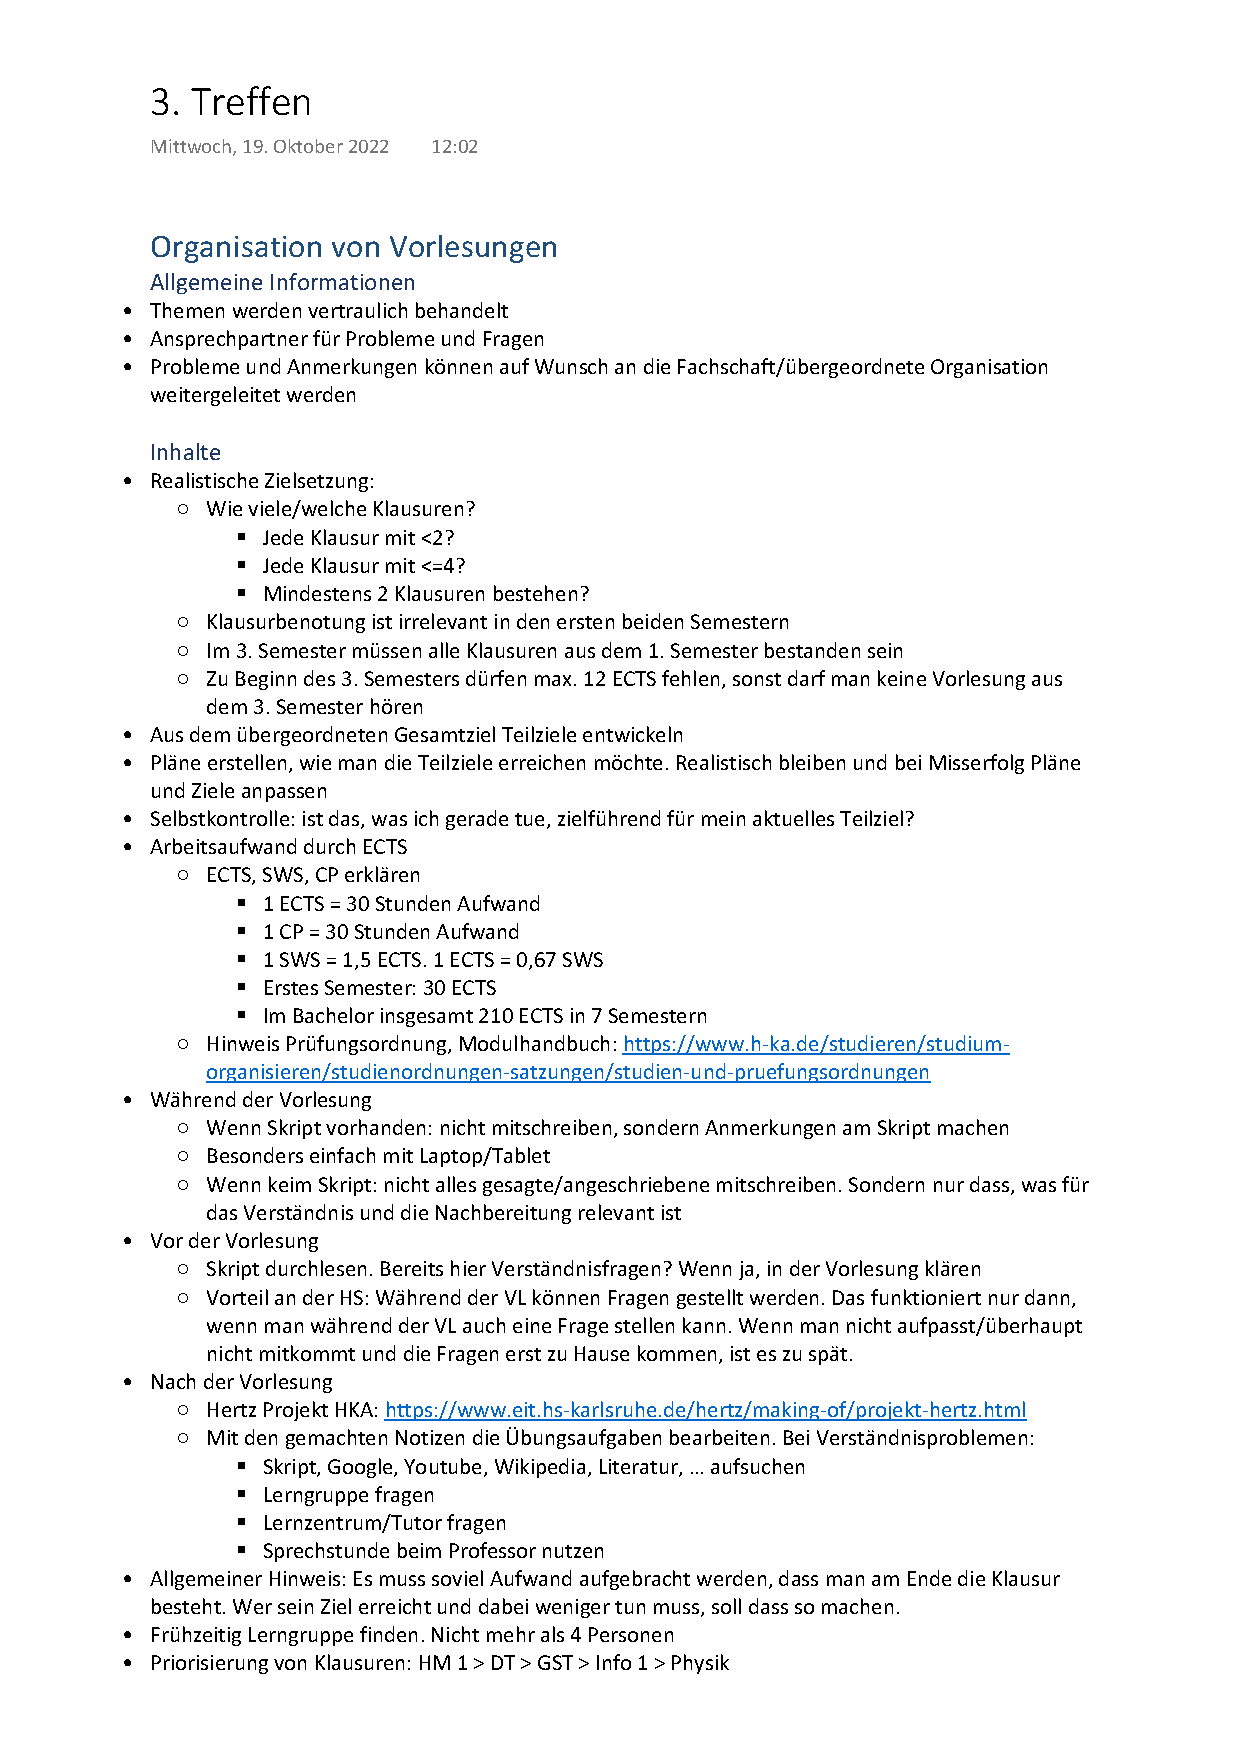
\includepdf[pages={1-2}]{treffen-3-ws22.pdf}
    \label{app:meeting3}

    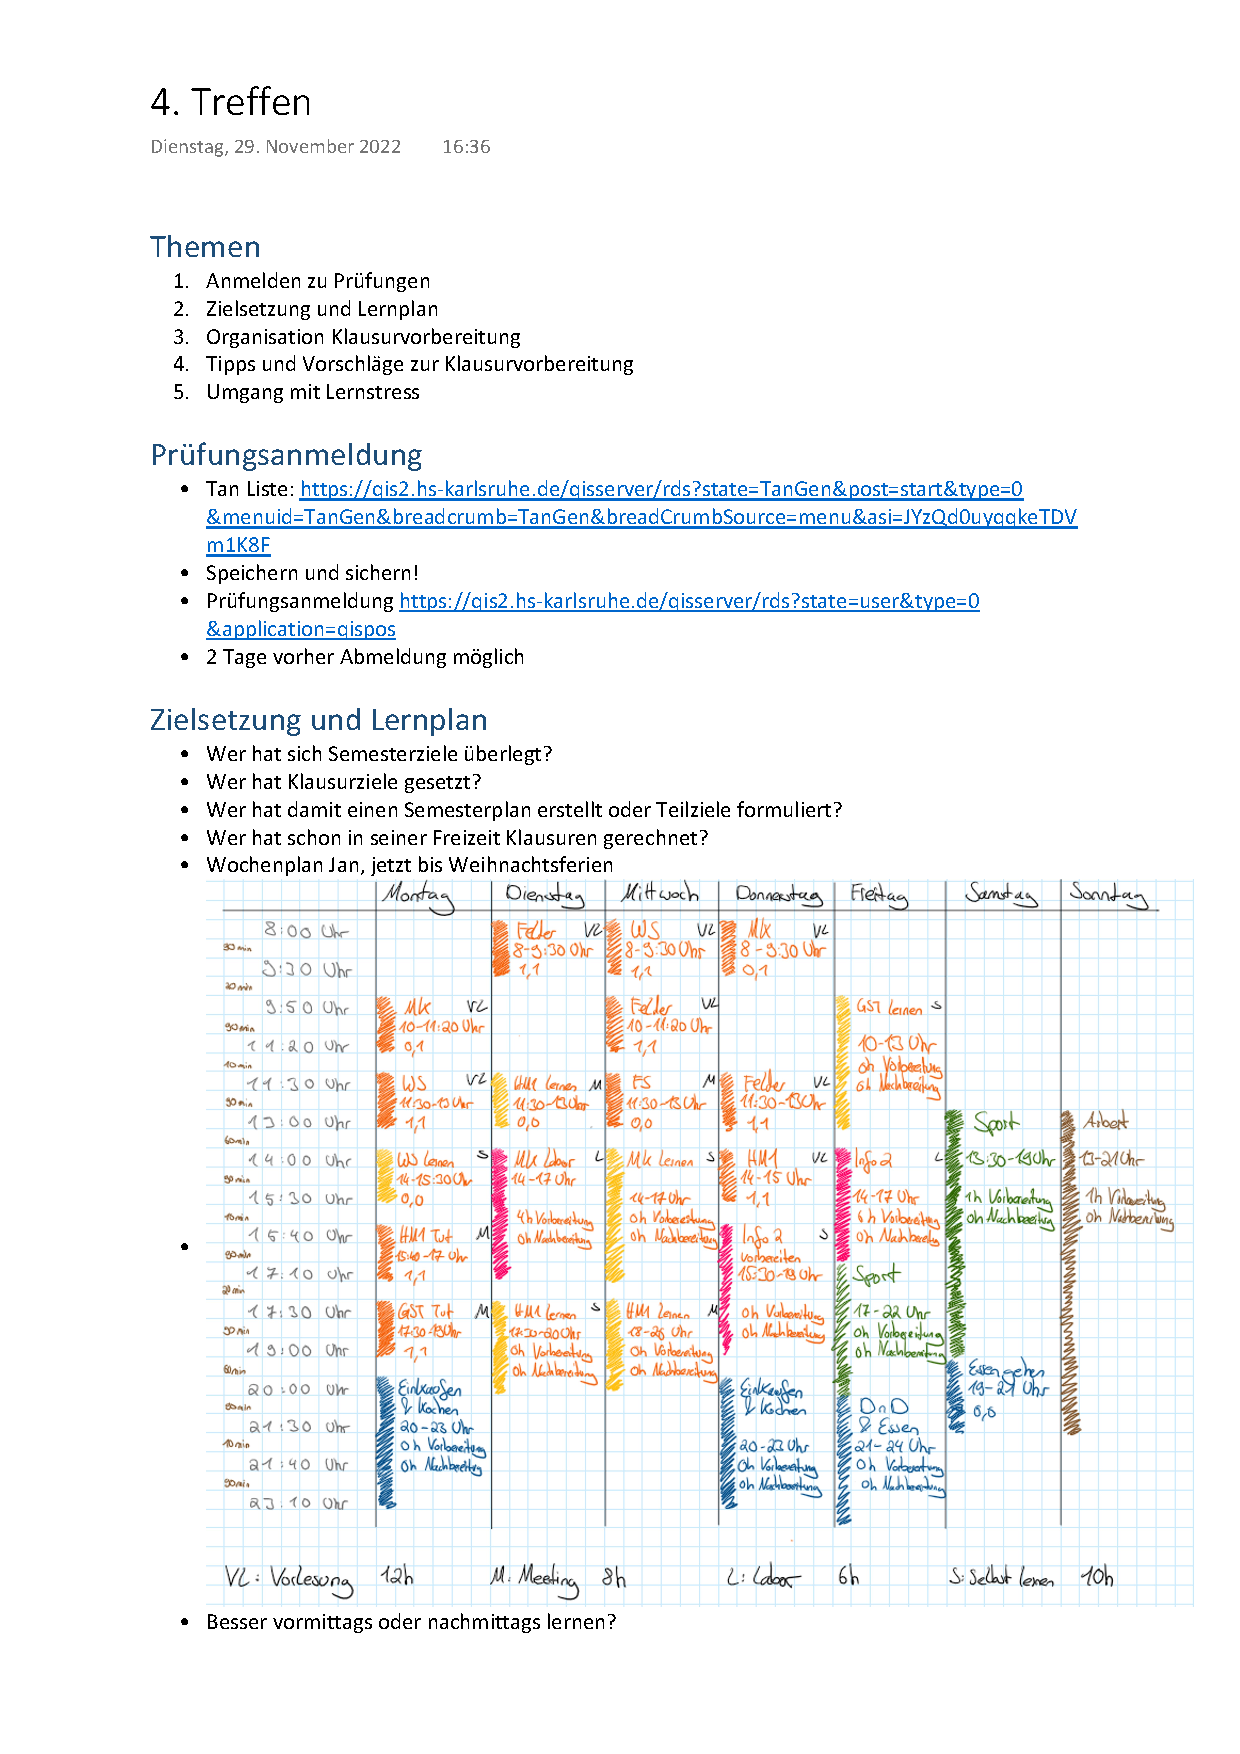
\includepdf[pages={1-3}]{treffen-4-ws22.pdf}
    \label{app:meeting4}

\end{document}